\section{Day 5}
\begin{tabular}{|c|c|}
\hline
Date: & 11.10.2013 \\
\hline
\end{tabular}
\subsection{MSC Office}
We set up at the Management Sciences of Health office. We met alot of new people. Mircel, I don't really know what he does yet. Think it was finance. Felix, good to meet him again. Bob the american. Cedrick and Emmir. Cedrick is a little shorter than Emir. And some other people.\\
\begin{figure}[p]
\centering
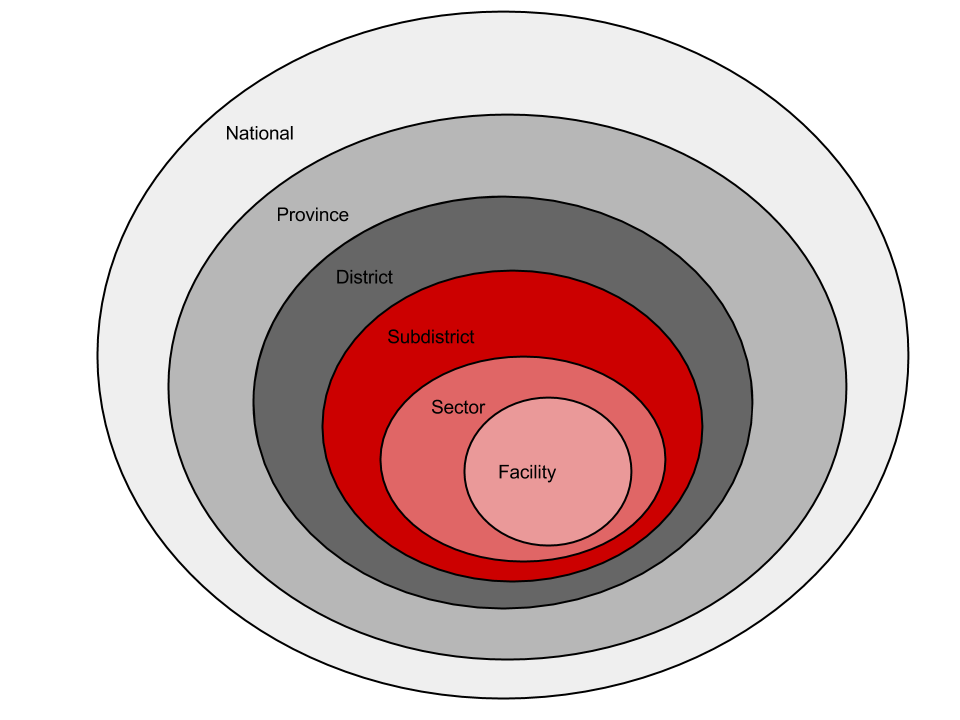
\includegraphics[width=15cm]{appendix/images/dhis2_rwanda_map_hierarchy}\\
\caption{Rwanda Map Hierarchy in DHIS2}
\label{Rwanda Map Hierarchy in DHIS2}
\end{figure}
\subsection{After Brunch}
After Randy's meeting we talked a little more about the projects that are relevant. The malaria surveliance and the interoperateabillity. I want the Malaria Surveliance. This would give us a concret assignment and a `know when its done' thing. The interoperateability would probably give us the best learning experience. Because it challenges me to think at computer systems at a higher level. I will send an email to Eric and discuss it further. I have a feeling I wont enjoy the best choice. Nappolina is the project manager.
\subsection{Conference room}
Randy gave us a briefing about the 2 remaining projects. This was alot of information to take in. 
\subsubsection{Malaria Active Surveliance}
The want to copy an existing report to a web based solution. Where this should be, I do not know.
\begin{itemize}
\item HTML
\item DHIS2
\item Mobile SMS
\item App
\end{itemize}
This was an extensive report. Randy proposed that we should mayby trim down the report a little. I think we've got the report on an email.
\subsubsection{Sentinal Surveliance}
This system is awsome. It's purpose is to collect weather and malaria data in order to see if theres an corelation between the two. They are going from 11 to 16 sentinels nationally. 
\begin{figure}[p]
\centering
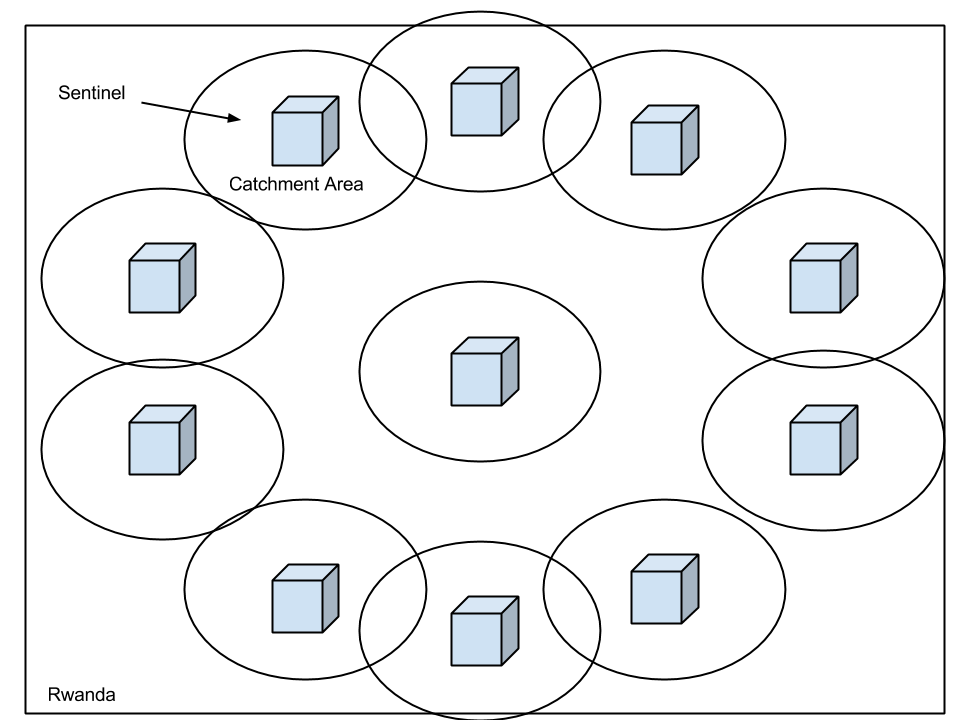
\includegraphics[width=15cm]{appendix/images/sentinel_surveliance}
\caption{Sentinel Surveliance}
\label{Sentinel Surveliance}
\end{figure}
\subsubsection{Ineroperateability}
Then got of to discuss the interoperateability project.
For starters Randy wanted to make a report based on some choosen indicators.
The task goes something like this.
\begin{enumerate}
\item Load data from dictionary
\item Choose indicators
\item Choose metadata/attributes
\item Produce report (Maybe with a preferred layout)
\end{enumerate}
He then explained how he wanted the entire system to work.
The result would be something like this.
\begin{figure}{p}
\centering
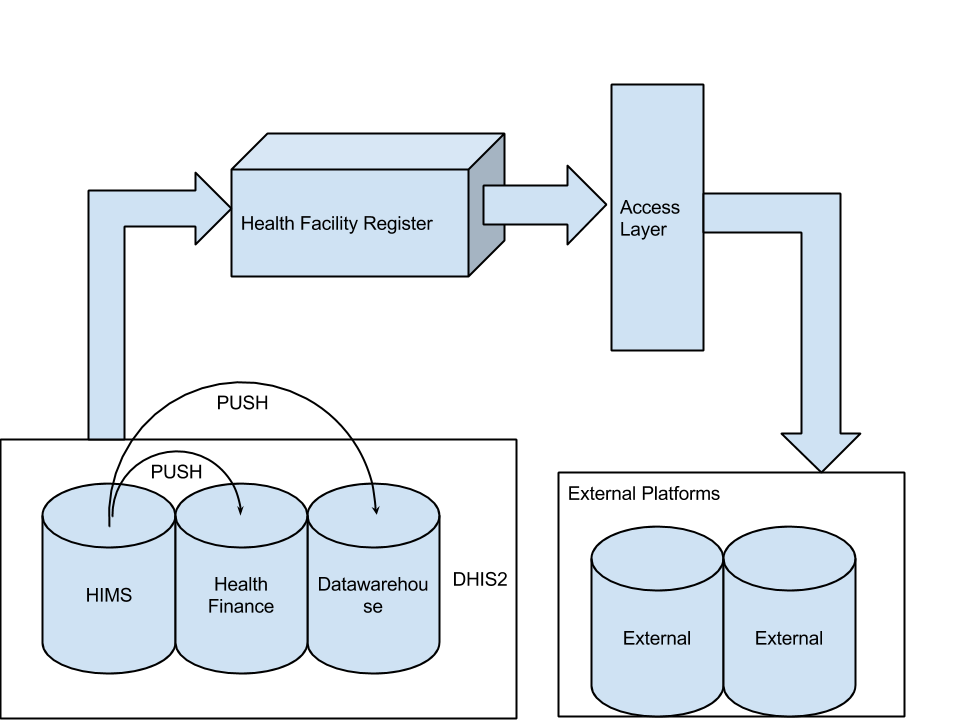
\includegraphics[width=15cm]{appendix/images/System_Architecture}
\caption{System Architecture}
\label{System Architecture}
\end{figure}
I think I should reaad up on SQL. It seem that this would be relevant.
For the last part he talked about how he would like to synchronize changes made to certain data element groups, cross instances of DHIS2. This in the case of adding adding elements. Would he like the same thin for indicators, I do not know. 
\subsection{Dinner at Randy's}


